% unit: u40
% sources: sources/009-final-exam.txt, sources/105-mit18-06scf11-final-exs-pdf-download-file.txt
\section{Final exam}\label{sec:u40}

A typical 18.06 final has nine questions in three closed-book hours, and this one runs the whole length of the course: from the special solutions of $A\vb{x}=\vb{0}$ through inverses, ranks, $A\T A$, Gram--Schmidt, projections and least squares, to eigenvalues, determinants and a recursion solved by a $2\times2$ eigenvalue problem. Most of the questions are posed with letters rather than numbers, so each is followed where useful by an example with numbers. The questions are grouped by theme; each is an exercise with its full solution. The reviews in Sections~\ref{sec:u37} and~\ref{sec:u39} cover the tools.

\subsection{Subspaces, ranks and one-sided inverses}

\begin{exercise}[Question 1]\label{exr:u40-q1}
$A$ is $3\times4$, and $A\vb{x}=\vb{0}$ has exactly two special solutions,
$\vb{x}_1=(1,1,1,0)$ and $\vb{x}_2=(-2,-1,0,1)$.
(a) Find the reduced row echelon form $R$ of $A$.
(b) Find the dimensions of $\Col{A}$, $\Nul{A}$, $\Col{A\T}$, $\Nul{A\T}$, and bases for those you can.
\end{exercise}
\begin{solution}
(a) A special solution sets one free variable to $1$ and the others to $0$. Here $\vb{x}_1$ has $(x_3,x_4)=(1,0)$ and $\vb{x}_2$ has $(x_3,x_4)=(0,1)$, so $x_3,x_4$ are free and $x_1,x_2$ are pivot variables. Two special solutions means $n-r=2$, so $r=2$ and the third row of $R$ is zero:
\[
R=\begin{bmatrix}1&0&*&*\\0&1&*&*\\0&0&0&0\end{bmatrix}.
\]
$R\vb{x}_1=\vb{0}$ gives $1+r_{13}=0$ and $1+r_{23}=0$; $R\vb{x}_2=\vb{0}$ gives $-2+r_{14}=0$ and $-1+r_{24}=0$. So
\[
R=\begin{bmatrix}1&0&-1&2\\0&1&-1&1\\0&0&0&0\end{bmatrix},
\]
whose free columns are the negatives of the pivot entries of the special solutions.

(b) $\dim\Nul{A}=n-r=2$, with basis $\vb{x}_1,\vb{x}_2$. $\dim\Col{A\T}=r=2$; elimination does not change the row space, so the nonzero rows of $R$, $(1,0,-1,2)$ and $(0,1,-1,1)$, are a basis (they are orthogonal to $\vb{x}_1$ and $\vb{x}_2$, as they must be). $\dim\Col{A}=r=2$, and the first two columns of $A$ (the pivot columns) are a basis, but we cannot write them down without $A$. $\dim\Nul{A\T}=m-r=1$: it is spanned by any nonzero vector orthogonal to the two pivot columns of $A$, again unknown.
\end{solution}

\begin{exercise}[Question 3]\label{exr:u40-q3}
(a) $A$ and $B$ have the same number of rows. Compare $\rank A$ with $\rank\begin{bmatrix}A&B\end{bmatrix}$.
(b) How do the ranks compare if $B=A^{2}$?
(c) If $A$ is $m\times n$ of rank $r$, what are the dimensions of $\Nul{A}$ and $\Nul{\begin{bmatrix}A&A\end{bmatrix}}$?
\end{exercise}
\begin{solution}
(a) Only $\rank A\le\rank\begin{bmatrix}A&B\end{bmatrix}$: the pivot columns of $A$ remain pivot columns of $\begin{bmatrix}A&B\end{bmatrix}$, and $B$ may contribute more. Both cases occur: with $A=\begin{bmatrix}1\\0\end{bmatrix}$, the rank stays $1$ for $B=A$ and jumps to $2$ for $B=\begin{bmatrix}0\\1\end{bmatrix}$.

(b) Equal. Column $j$ of $A^{2}$ is $A$ times column $j$ of $A$, a combination of the columns of $A$. So $\Col{\begin{bmatrix}A&A^{2}\end{bmatrix}}=\Col{A}$ and no new pivot columns appear.

(c) $\dim\Nul{A}=n-r$. The block matrix $\begin{bmatrix}A&A\end{bmatrix}$ is $m\times2n$, and its last $n$ columns repeat the first $n$, so its rank is still $r$ and its nullspace has dimension $2n-r$. (It contains every $(\vb{y},-\vb{y})$, an $n$-dimensional family, plus $(\vb{z},\vb{0})$ for $\vb{z}\in\Nul{A}$.)
\end{solution}

\begin{exercise}[Question 4]\label{exr:u40-q4}
$A$ is $5\times3$ and $A\vb{x}\neq\vb{0}$ whenever $\vb{x}\neq\vb{0}$.
(a) What can you say about the columns of $A$?
(b) Show that $A\T A\vb{x}=\vb{0}$ only for $\vb{x}=\vb{0}$ by explaining the key step: if $A\T A\vb{x}=\vb{0}$ then $\vb{x}\T A\T A\vb{x}=0$, and then (why?) $A\vb{x}=\vb{0}$.
(c) So $A\T A$ is invertible. Why is $B=(A\T A)^{-1}A\T$ a one-sided inverse of $A$, on which side, and why is it not two-sided?
\end{exercise}
\begin{solution}
(a) $\Nul{A}=\{\vb{0}\}$, so the three columns are independent: full column rank, $r=n=3$.
(b) $\vb{x}\T A\T A\vb{x}=(A\vb{x})\T(A\vb{x})=\|A\vb{x}\|^{2}$, the squared length of $A\vb{x}$. A vector of length zero is the zero vector, so $A\vb{x}=\vb{0}$, and by (a) $\vb{x}=\vb{0}$.
(c) $BA=(A\T A)^{-1}(A\T A)=I_3$: $B$ is a left inverse. It cannot be a right inverse: $AB$ is $5\times5$ but has rank at most $3$, so $AB\neq I_5$. In fact $AB=A(A\T A)^{-1}A\T$ is the projection onto the three-dimensional column space of $A$ (Theorem~\ref{thm:u36-left}).
\end{solution}

\subsection{An inverse that stays triangular}

\begin{exercise}[Question 2]\label{exr:u40-q2}
(a) Find the inverse of $U=\begin{bmatrix}a&b&c\\0&d&e\\0&0&f\end{bmatrix}$, all entries nonzero.
(b) The columns of $U$ are eigenvectors of a matrix $A$. Show that $A$ is upper triangular.
(c) Explain why this $U$ cannot be the first factor in an SVD $A=U\Sigma V\T$.
\end{exercise}
\begin{solution}
(a) Gauss--Jordan on $\begin{bmatrix}U&I\end{bmatrix}$. Divide the rows by $a$, $d$, $f$:
\[
\left[\begin{array}{ccc|ccc}1&b/a&c/a&1/a&0&0\\0&1&e/d&0&1/d&0\\0&0&1&0&0&1/f\end{array}\right].
\]
Subtract $e/d$ times row 3 from row 2 and $c/a$ times row 3 from row 1, then $b/a$ times the new row 2 from row 1:
\[
U^{-1}=\begin{bmatrix}1/a&-b/(ad)&(be-cd)/(adf)\\0&1/d&-e/(df)\\0&0&1/f\end{bmatrix}.
\]
(The $(1,3)$ entry is $-\frac{c}{af}+\frac{b}{a}\cdot\frac{e}{df}=\frac{be-cd}{adf}$.) Cofactors give the same answer: $U^{-1}=C\T/\det U$ with $\det U=adf$.

(b) Three independent eigenvectors diagonalize $A$: $A=U\Lambda U^{-1}$. $U$, $\Lambda$ and (by part (a)) $U^{-1}$ are all upper triangular, and products of upper triangular matrices are upper triangular.

(c) The $U$ of an SVD has orthonormal columns. Here the first two columns have dot product $ab+0\cdot d+0\cdot0=ab\neq0$.
\end{solution}

\begin{example}[Question 2 with numbers]\label{ex:u40-tri}
For $U=\begin{bmatrix}1&2&3\\0&4&5\\0&0&6\end{bmatrix}$ ($a,b,c,d,e,f=1,2,3,4,5,6$) the formula gives
\[
U^{-1}=\begin{bmatrix}1&-\tfrac{2}{4}&\tfrac{2\cdot5-3\cdot4}{1\cdot4\cdot6}\\0&\tfrac14&-\tfrac{5}{24}\\0&0&\tfrac16\end{bmatrix}=\begin{bmatrix}1&-\tfrac12&-\tfrac{1}{12}\\0&\tfrac14&-\tfrac{5}{24}\\0&0&\tfrac16\end{bmatrix}.
\]
Check the last column of $UU^{-1}$: row 1 gives $-\tfrac{1}{12}-\tfrac{10}{24}+\tfrac36=\tfrac{-2-10+12}{24}=0$, row 2 gives $-\tfrac{20}{24}+\tfrac56=0$, row 3 gives $1$.
\end{example}

\subsection{Energy in an eigenvector basis}

\begin{exercise}[Question 5]\label{exr:u40-q5}
$A$ is $3\times3$ symmetric positive definite, $A\vb{q}_i=\lambda_i\vb{q}_i$ with orthonormal $\vb{q}_i$ and $0<\lambda_1<\lambda_2<\lambda_3$. Let $\vb{x}=c_1\vb{q}_1+c_2\vb{q}_2+c_3\vb{q}_3$.
(a) Compute $\vb{x}\T\vb{x}$ and $\vb{x}\T A\vb{x}$ in terms of the $c$'s and $\lambda$'s.
(b) Which $c$'s make the ratio $\vb{x}\T A\vb{x}/\vb{x}\T\vb{x}$ as large as possible?
\end{exercise}
\begin{solution}
(a) Expanding $(c_1\vb{q}_1+c_2\vb{q}_2+c_3\vb{q}_3)\T(c_1\vb{q}_1+c_2\vb{q}_2+c_3\vb{q}_3)$ gives nine terms $c_ic_j\vb{q}_i\T\vb{q}_j$; orthonormality keeps only $i=j$, each with $\vb{q}_i\T\vb{q}_i=1$:
\[
\vb{x}\T\vb{x}=c_1^{2}+c_2^{2}+c_3^{2}.
\]
Since $A\vb{x}=c_1\lambda_1\vb{q}_1+c_2\lambda_2\vb{q}_2+c_3\lambda_3\vb{q}_3$, the same expansion gives
\[
\vb{x}\T A\vb{x}=\lambda_1c_1^{2}+\lambda_2c_2^{2}+\lambda_3c_3^{2}.
\]
(b) The ratio is a weighted average of the $\lambda$'s with weights $c_i^{2}/\sum c_j^{2}$, so
\[
\frac{\vb{x}\T A\vb{x}}{\vb{x}\T\vb{x}}=\frac{\lambda_1c_1^{2}+\lambda_2c_2^{2}+\lambda_3c_3^{2}}{c_1^{2}+c_2^{2}+c_3^{2}}\le\frac{\lambda_3(c_1^{2}+c_2^{2}+c_3^{2})}{c_1^{2}+c_2^{2}+c_3^{2}}=\lambda_3,
\]
with equality exactly when $c_1=c_2=0$. The ratio is largest when $\vb{x}$ is a multiple of the top eigenvector $\vb{q}_3$, and its maximum value is $\lambda_3$. This ratio is the \emph{Rayleigh quotient}; maximizing it numerically is one way to find the largest eigenvalue.
\end{solution}

\begin{example}[The Rayleigh quotient of a $2\times2$ matrix]\label{ex:u40-rayleigh}
For $A=\begin{bmatrix}2&1\\1&2\end{bmatrix}$ ($\lambda=1,3$; $\vb{q}=\tfrac{1}{\sqrt2}(1,-1),\tfrac{1}{\sqrt2}(1,1)$) take unit vectors $\vb{x}=(\cos\theta,\sin\theta)$. Then
\[
\vb{x}\T A\vb{x}=2\cos^{2}\theta+2\cos\theta\sin\theta+2\sin^{2}\theta=2+\sin2\theta,
\]
which ranges between $1$ and $3$. The maximum $3=\lambda_2$ occurs at $\theta=\pi/4$, the direction of $(1,1)$, and the minimum $1=\lambda_1$ at $\theta=3\pi/4$, the direction of $(-1,1)$ (Figure~\ref{fig:u40-rayleigh}).
\end{example}

\begin{figure}[ht]\centering
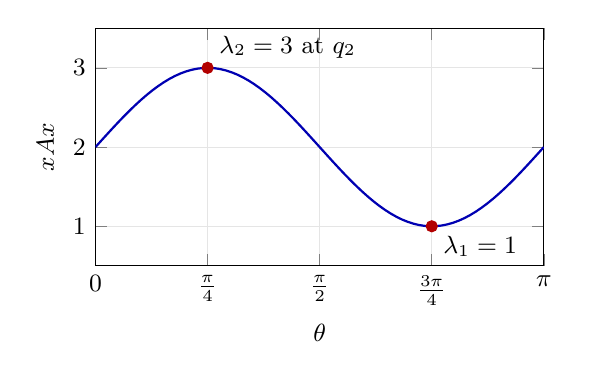
\begin{tikzpicture}
\begin{axis}[width=0.6\textwidth,height=4.6cm,xlabel={$\theta$},ylabel={$\vb{x}\T A\vb{x}$},
  xmin=0,xmax=3.1416,ymin=0.5,ymax=3.5,xtick={0,0.7854,1.5708,2.3562,3.1416},
  xticklabels={$0$,$\frac{\pi}{4}$,$\frac{\pi}{2}$,$\frac{3\pi}{4}$,$\pi$},ytick={1,2,3},grid=major,grid style={gray!20},font=\small]
\addplot[blue!70!black,thick,domain=0:3.1416,samples=80] {2+sin(deg(2*x))};
\addplot[only marks,mark=*,red!70!black] coordinates {(0.7854,3) (2.3562,1)};
\node[above right,font=\small] at (axis cs:0.80,3) {$\lambda_2=3$ at $\vb{q}_2$};
\node[below right,font=\small] at (axis cs:2.37,1) {$\lambda_1=1$};
\end{axis}
\end{tikzpicture}
\caption{The Rayleigh quotient $\vb{x}\T A\vb{x}$ on unit vectors $\vb{x}=(\cos\theta,\sin\theta)$ for $A=\begin{bmatrix}2&1\\1&2\end{bmatrix}$. Its maximum and minimum are the eigenvalues, reached at the eigenvectors.}\label{fig:u40-rayleigh}
\end{figure}

\subsection{Gram--Schmidt, projections and least squares}

\begin{exercise}[Question 6]\label{exr:u40-q6}
(a) Find a combination $\vb{w}$ of the independent vectors $\vb{v}$ and $\vb{u}$ that is perpendicular to $\vb{u}$.
(b) For $A=\begin{bmatrix}\vb{u}&\vb{v}\end{bmatrix}$ find $Q$ (orthonormal columns) and $R$ ($2\times2$ upper triangular) with $A=QR$.
(c) Using only $Q$, find the projection matrix onto the plane spanned by $\vb{u}$ and $\vb{v}$.
\end{exercise}
\begin{solution}
(a) $\vb{w}=\vb{0}$ is perpendicular to everything, but the useful answer subtracts from $\vb{v}$ just enough of $\vb{u}$: $\vb{w}=\vb{v}-c\vb{u}$ with $0=\vb{u}\T\vb{w}=\vb{u}\T\vb{v}-c\,\vb{u}\T\vb{u}$, so
\[
\vb{w}=\vb{v}-\frac{\vb{u}\T\vb{v}}{\vb{u}\T\vb{u}}\,\vb{u}.
\]
(b) Normalize: $\vb{q}_1=\vb{u}/\|\vb{u}\|$, $\vb{q}_2=\vb{w}/\|\vb{w}\|$. Then $\vb{u}=\|\vb{u}\|\vb{q}_1$ and $\vb{v}=\vb{w}+c\vb{u}=c\|\vb{u}\|\vb{q}_1+\|\vb{w}\|\vb{q}_2$, so
\[
A=\begin{bmatrix}\vb{u}&\vb{v}\end{bmatrix}=\begin{bmatrix}\vb{q}_1&\vb{q}_2\end{bmatrix}\begin{bmatrix}\|\vb{u}\|&c\|\vb{u}\|\\0&\|\vb{w}\|\end{bmatrix}=QR,\qquad c=\frac{\vb{u}\T\vb{v}}{\vb{u}\T\vb{u}}.
\]
(c) $P=A(A\T A)^{-1}A\T$ with $A=QR$ and $Q\T Q=I$:
\[
P=QR\,(R\T Q\T QR)^{-1}R\T Q\T=QR\,R^{-1}(R\T)^{-1}R\T Q\T=QQ\T.
\]
\end{solution}

\begin{figure}[ht]\centering
\begin{tikzpicture}[scale=1.4,>=Stealth,font=\small]
  \draw[->,very thick,blue!70!black] (0,0) -- (3,0) node[below right] {$\vb{u}$};
  \draw[->,very thick,orange!80!black] (0,0) -- (2.2,1.8) node[above] {$\vb{v}$};
  \draw[->,thick,blue!50] (0,0) -- (2.2,0) node[pos=0.55,below] {$c\vb{u}$};
  \draw[->,thick,red!70!black] (2.2,0) -- (2.2,1.8) node[pos=0.5,right] {$\vb{w}=\vb{v}-c\vb{u}$};
  \draw[->,thick,red!70!black,dashed] (0,0) -- (0,1.8) node[left] {$\vb{w}$};
  \draw (2.2,0.22) -- (1.98,0.22) -- (1.98,0);
  \draw[gray,dotted] (0,1.8) -- (2.2,1.8);
\end{tikzpicture}
\caption{Gram--Schmidt in Question 6: subtract from $\vb{v}$ its projection $c\vb{u}$ onto $\vb{u}$; what remains, $\vb{w}$, is perpendicular to $\vb{u}$. Normalizing $\vb{u}$ and $\vb{w}$ gives $Q$.}\label{fig:u40-gs}
\end{figure}

\begin{example}[Question 6 with numbers]\label{ex:u40-qr}
Take $\vb{u}=(1,2,2)$ and $\vb{v}=(5,1,1)$. Then $c=\vb{u}\T\vb{v}/\vb{u}\T\vb{u}=9/9=1$ and $\vb{w}=\vb{v}-\vb{u}=(4,-1,-1)$, which is perpendicular to $\vb{u}$ ($4-2-2=0$). With $\|\vb{u}\|=3$ and $\|\vb{w}\|=\sqrt{18}=3\sqrt2$:
\[
Q=\begin{bmatrix}1/3&4/(3\sqrt2)\\2/3&-1/(3\sqrt2)\\2/3&-1/(3\sqrt2)\end{bmatrix},\qquad R=\begin{bmatrix}3&3\\0&3\sqrt2\end{bmatrix}.
\]
Check the second column: $3\vb{q}_1+3\sqrt2\,\vb{q}_2=(1,2,2)+(4,-1,-1)=(5,1,1)=\vb{v}$. The projection onto the plane is
\[
P=QQ\T=\begin{bmatrix}1&0&0\\0&1/2&1/2\\0&1/2&1/2\end{bmatrix},
\]
which makes sense: both $\vb{u}$ and $\vb{v}$ have equal second and third entries, so the plane is $\{x_2=x_3\}$, and $P$ keeps $x_1$ and averages $x_2$ with $x_3$.
\end{example}

\begin{exercise}[Question 8]\label{exr:u40-q8}
$A$ has independent columns.
(a) Give formulas for the least-squares solution $\hat{\vb{x}}$ of $A\vb{x}=\vb{b}$ and for $\vb{p}=A\hat{\vb{x}}$.
(b) In which fundamental subspaces are $\vb{p}$ and $\vb{e}=\vb{b}-\vb{p}$?
(c) Find the projection matrix onto the column space of $A=\begin{bmatrix}1&0\\3&0\\0&-1\\0&-3\end{bmatrix}$.
\end{exercise}
\begin{solution}
(a) Multiply $A\vb{x}=\vb{b}$ by $A\T$ to get the normal equations $A\T A\hat{\vb{x}}=A\T\vb{b}$; $A\T A$ is invertible because the columns are independent, so
\[
\hat{\vb{x}}=(A\T A)^{-1}A\T\vb{b},\qquad \vb{p}=A\hat{\vb{x}}=A(A\T A)^{-1}A\T\vb{b}.
\]
(b) $\vb{p}$ is a combination of the columns, so $\vb{p}\in\Col{A}$. The error is perpendicular to the column space, so $\vb{e}\in\Nul{A\T}$; the normal equations say exactly $A\T\vb{e}=\vb{0}$.
(c) The columns are orthogonal: $A\T A=\begin{bmatrix}10&0\\0&10\end{bmatrix}=10I$. Hence
\[
P=A(10I)^{-1}A\T=\frac{1}{10}AA\T=\frac{1}{10}\begin{bmatrix}1&3&0&0\\3&9&0&0\\0&0&1&3\\0&0&3&9\end{bmatrix},
\]
the sum of the projections onto the two orthogonal columns.
\end{solution}

\subsection{Permutations, determinants and a recursion}

\begin{exercise}[Question 7]\label{exr:u40-q7}
Let $C=\begin{bmatrix}0&0&0&1\\1&0&0&0\\0&1&0&0\\0&0&1&0\end{bmatrix}$, so $C^{2}=\begin{bmatrix}0&0&1&0\\0&0&0&1\\1&0&0&0\\0&1&0&0\end{bmatrix}$.
(a) Find the eigenvalues of $C$ and $C^{2}$.
(b) Find $C^{-1}$ and $(C^{2})^{-1}$.
(c) Find $\det C$, $\det(C+I)$ and $\det(C+2I)$.
\end{exercise}
\begin{solution}
(a) Expanding $\det(C-\lambda I)$ by cofactors gives $\lambda^{4}-1=(\lambda-1)(\lambda+1)(\lambda^{2}+1)$, so $\lambda=1,-1,i,-i$, the four fourth roots of $1$. (A quicker route: $C$ moves each entry down one place cyclically, so $C^{4}=I$ and every eigenvalue satisfies $\lambda^{4}=1$; check that all four occur.) The eigenvalues of $C^{2}$ are the squares: $1,1,-1,-1$. The eigenvectors are the Fourier vectors $(1,\bar\lambda,\bar\lambda^{2},\bar\lambda^{3})$ of Section~\ref{sec:u30}.

(b) Permutation matrices are orthogonal, so $C^{-1}=C\T=\begin{bmatrix}0&1&0&0\\0&0&1&0\\0&0&0&1\\1&0&0&0\end{bmatrix}$. $C^{2}$ exchanges entries $1\leftrightarrow3$ and $2\leftrightarrow4$, so it is its own inverse: $(C^{2})^{-1}=C^{2}$.

(c) $\det C=1\cdot(-1)\cdot i\cdot(-i)=-1$. Adding $I$ adds $1$ to each eigenvalue, so $\det(C+I)=2\cdot0\cdot(1+i)(1-i)=0$; adding $2I$ gives $\det(C+2I)=3\cdot1\cdot(2+i)(2-i)=3\cdot5=15$. Equivalently, set $\lambda=-1$ and $\lambda=-2$ in $\det(C-\lambda I)=\lambda^{4}-1$: $1-1=0$ and $16-1=15$.
\end{solution}

\begin{exercise}[Question 9]\label{exr:u40-q9}
$A_n$ is the $n\times n$ tridiagonal matrix with $3$ on the diagonal, $2$ above it and $1$ below it; $D_n=\det A_n$.
(a) Find $D_2$ and $D_3$.
(b) Use cofactors of row 1 and column 1 to find $a,b$ in $D_n=aD_{n-1}+bD_{n-2}$.
(c) Writing the recursion as $\begin{bmatrix}D_n\\D_{n-1}\end{bmatrix}=\begin{bmatrix}a&b\\1&0\end{bmatrix}\begin{bmatrix}D_{n-1}\\D_{n-2}\end{bmatrix}$, how fast does $D_n$ grow? Find $D_5$.
\end{exercise}
\begin{solution}
(a) $D_1=3$, $D_2=\det\begin{bmatrix}3&2\\1&3\end{bmatrix}=9-2=7$, and $D_3=3D_2-2\cdot1\cdot D_1=21-6=15$ (by the expansion in (b)).

(b) Expand along row 1. The $(1,1)$ cofactor is $D_{n-1}$. The $(1,2)$ entry is $2$ with sign $-$, and its minor (delete row 1, column 2) has first column $(1,0,\dots,0)$; expanding that minor down its first column leaves $1\cdot D_{n-2}$. So
\[
D_n=3D_{n-1}-2D_{n-2},\qquad a=3,\ b=-2.
\]
(c) The matrix $\begin{bmatrix}3&-2\\1&0\end{bmatrix}$ has trace $3$ and determinant $2$, so $\lambda^{2}-3\lambda+2=0$ and $\lambda=1,2$. Powers of this matrix grow like $2^{n}$, so $D_n$ grows like $2^{n}$. Matching $D_n=\alpha2^{n}+\beta$ to $D_1=3$, $D_2=7$ gives $\alpha=2$, $\beta=-1$:
\[
D_n=2^{n+1}-1,\qquad D_4=31,\qquad D_5=3\cdot31-2\cdot15=63=2^{6}-1.
\]
\end{solution}

\begin{trap}
Carry the sign of $b$ through. Writing the recursion as $D_n=3D_{n-1}+2D_{n-2}$ gives $D_5=207$, which is wrong: a direct computation of $\det A_5$ gives $63$, and the sign comes from the checkerboard $(-1)^{1+2}$ in the cofactor of the $(1,2)$ entry. Checking a small case ($D_3=15$ from the formula against $\det A_3$ by elimination) catches this kind of slip.
\end{trap}
